%Every LaTeX file needs a documentclass declaration.
%Possibilities are article, book, letter.  Font size is also declared.

\documentclass[10pt]{article}

%special packages used for symbols, formatting, etc.

\usepackage{amsmath} % contains the align* environment, which is great for manipulating formulas
\usepackage{amssymb} % contains common symbols
\usepackage{amsthm} % has the proof environment
\usepackage[margin=1in]{geometry} % specifies page properties, such as the margin
%\usepackage{siunitx} % useful for typesetting units
\usepackage{tikz} % useful for graphics
\usepackage{xcolor}

% Define a lemma environment
% Set the style of the new theorem environments so that the text isn't in italics
\theoremstyle{definition}
% Define lemma environment, the first argument is the name in LaTeX, the second argument is what is typeset
\newtheorem{lemma}{Lemma}

% User-defined commands

\newcommand{\newprob}{\medskip \hrule \medskip}
\newcommand{\fanc}[1]{\mathbb{#1}}
\newcommand{\rn}[1]{\fanc{R}^{#1}}
\def\qed{\hspace*{\fill}\rule{1.854mm}{3mm}}  % the fancy box at the end of a proof

%%%%%%%%%%%%%%%%%%%%%%%%%%%%%%%%%%%%%%%%%%%%%%

%beginning of document, every \begin{} also requires an \end{} command.

%\renewcommand{\baselinestretch}{2}

\begin{document}

\pagestyle{empty}  %suppress page numbers, etc.

\begin{center}  %center command, also see flushright, flushleft

{\bf MATH 423-01  Advanced Calculus I

Homework \#5

Assigned: September 30, 2022

Due: October 7, 2022

\textcolor{red}{What to finish: 1abc, 2abcdef, 3, 5, 6, 8ab, 9abcd}
}

\end{center}

\medskip

\hrule   %horizontal line

\bigskip

% list environment: description, itemize, and enumerate

\begin{enumerate}

%%%%%%%%%%%%%%%%%%%%%%

\item  ~[Nupen, R.] Consider the sequence defined by $x_1 = 3$ and $$x_{n+1} = \frac{1}{4-x_n}.$$

	\begin{enumerate}
	
	\item  Prove that $(x_n)$ converges.  Hint: this sequence is defined recursively, so using an argument with $\varepsilon$ won't work.  Instead use induction and the Monotone Convergence Theorem.
	
	\item  Now we know that $\lim{(x_n)} = x$, $\exists x \in \mathbb{R}$.  Explain why $\lim{(x_{n+1})}$ must also exist and $\lim{(x_{n+1})} = x$.
	
	\item  Take the limit of both sides of the recursive definition in (a) to explicitly compute $x$.
	
	\end{enumerate}
	
%%%%%%%%%%%%

\item  ~[Griffith, B.] Let $(a_n)$ be a bounded sequence.

	\begin{enumerate}
	
	\item  Consider the sequence defined by $b_n = \sup{\left(\{ a_k : k \geq n \} \right)}$.  If $a_n = \frac{(-1)^n}{n}$, for $n \in \mathbb{N}$, compute the first ten terms of $b_n$.  What is $\lim{(b_n)}$?
	
	\item  Prove that for any bounded sequence, $(a_n)$, the sequence defined by $b_n = \sup{\left(\{ a_k : k \geq n \} \right)}$ converges.  This is not a specific statement about the example sequence in (a) but a general statement about all sequences $(a_n)$ and $(b_n)$.  Hint: use the Monotone Convergence Theorem.
	
	\item  The \emph{limit superior} of $(a_n)$, or $\limsup{(a_n)}$, is defined by $$\limsup{(a_n)} = \lim{(b_n)},$$ where is the sequence defined in (a).  Provide a reasonable definition for the \emph{limit inferior}, $\liminf{(a_n)}$, and briefly explain why it always exists for any bounded sequence.
	
	\item  Calculate the first ten terms for your new sequence you defined in (c) using $(a_n)$ from (a), and then calculate $\liminf{(a_n)}$.
	
	\item  Prove that $\liminf{(a_n)} \leq \limsup{(a_n)}$ for every bounded sequence, and give an example of a sequence for which the inequality is strict.
	
	\item  Show that $\liminf{(a_n)} = \limsup{(a_n)}$ if and only if $\lim{(a_n)}$ exists.  In this case all three values are the same.  Hint: use (e) and the Squeeze Theorem for one direction, and use (b) and the Cauchy Criterion for the other direction.  One of these directions is considerably harder than the other.
	
	\end{enumerate}
	
%%%%%%%%%%%%%%%%

\item  ~[Papiernik, J.] Prove that subsequences of a convergent sequence converge to the same limit as the original sequence.
	
%%%%%%%%%%%%%%

\item  ~[Powers, S.] Give an example of each of the following, or argue that such a request is impossible.

	\begin{enumerate}
	
	\item  A sequence that does not contain $0$ or $1$ as a term but contains subsequences converging to each of these values.
 
 \textbf{\underline{Answer:}}
 \textcolor{black}{Consider the sequence $(a_n)$ given by $(a_n) = (1+\frac{1}{n}$ if $n$ is odd, $\frac{1}{n}$ if $n$ is even.  Clearly, $(1+\frac{1}{n})! \rightarrow 1 and (\frac{1}{n})! \rightarrow 0$, so the subsequence of odd terms converges to 1 and the subsequence of even terms converges to 0, even though neither 1 nor 0 appear as terms of the sequence.} 
	
	\item  A monotone sequence that diverges but has a convergent subsequence.
	
 \textbf{\underline{Answer:}}
 \textcolor{black}{This is impossible.  To see why, suppose $(a_n)$ is a monotone sequence with a convergent subsequence $(a_{nk})$. In fact, for simplicity, assume $(a_n)$ is increasing. Since $(a_{nk})$ converges, it must be bounded, so there exists $M \in \mathbb{R}$ such that $(a_{nk}) \leq M$ for all of the $a_{nk}$ . Now, for any term $a_n$ from the original sequence, there exists $k \in \mathbb{N}$ such that $nk > n$; then $a_1 \leq a_n \leq a_{nk} \leq M$. Since our choice of $n$ was arbitrary, we see that $a_1 \leq a_n \leq M$ for all $n \in {1, 2, 3, . . .}$, so the sequence $(a_n)$ must be bounded. A similar argument works when $(a_n)$ is decreasing. Therefore, any monotone sequence with a convergent subsequence must be bounded and, therefore, convergent by the Monotone Convergence Theorem. }
	\item  A sequence that contains subsequences converging to every point in the infinite set $\left\{ 1, \frac{1}{2}, \frac{1}{3}, \frac{1}{4}, \ldots \right\}$.
 
  \textbf{\underline{Answer:}}
 \textcolor{black}{Consider the sequence $\left\{1, 1, \frac{1}{2}, 1, \frac{1}{2}, \frac{1}{3},...\right\}$  Then the subseqeuences must converge to $1$, $\frac{1}{2}$, $\frac{1}{3}$,....}
	
	\item  An unbounded sequence with a convergent subsequence.
 
	\textbf{\underline{Answer:}}
 \textcolor{black}{Let
$a_n =(n$ if n is even, $0$ if n is odd). Then $(a_n)$ in an unbounded sequence with the convergent subsequence $(a_{2k-1})^{\infty}_{k=1}$.
 }

 
	\item  A sequence that has a subsequence that is bounded but contains no subsequence that converges.

 \textbf{\underline{Answer:}}
 \textcolor{black}{This is false. Because by Bolzano-Weirstrass theorem, every bounded sequence has a convergent subsequence.}
 
	\end{enumerate}
	
%%%%%%%%%%%%
	
\item  ~[Schipke, K.] Assume $(a_n)$ is a bounded sequence with the property that every convergent subsequence of $(a_n)$ converges to the same limit $a \in \mathbb{R}$.  Prove that $(a_n)$ converges to $a$.  Hint: use contradiction, but note that there are two cases to consider.

\newpage
	
%%%%%%%%%%%%%

\item  ~[Schmidt, S.] Let $(a_n)$ be a bounded sequence, and define the set $$S = \{ x \in \mathbb{R}: x < a_n \textnormal{ for infinitely many terms of } a_n \}.$$  Show that there exists a subsequence of $(a_n)$ converging to $s = \sup{(S)}$.  This is another proof of the Bolzano-Weierstrass Theorem that uses the Axiom of Completeness.  Hint: use the lemma that relates the supremum to $\varepsilon$.  I used $\frac{1}{k}$, for $k \in \mathbb{N}$, for the $\varepsilon$ in the lemma, so that I could choose an appropriate term for $a_{n_k}$ from the infinite choices $S$ provides.
\begin{proof}
This is a direct approach to the Bolzano-Weierstrass Theorem when using the supremum, both parts of its definition-it's an upper bound, and it's the least of such-almost are always used.  Let $\existk \in \mathbb{N}$.  And since $s=sup(S)$ and $\frac{s-1}{k}<s$, $s$ cannot be an upper bound of $S$.  This is from the definition of the supremum..  Supremum is the least upper bound, so anything strictly less than the supremum cannot be an upper bound at all.  So, we have an $x \in S$ for which $x>\frac{s-1}{k}$.  From the definition of $S$, there are infinitely many $a_n$ greater than this $x$, and hence also greater that $\fract{s-1}{k}$.  So by the definition of the supremum, anything strictly greater than the supremum is strictly greater than all of the elements of the set.  So, we have $\frac{s+1}{k}$ is greater than all of S, and in particular, it is not in $S$.  From the definition of $S$, there are only finitely many $a_n > \frac{s+1}{k}$, so there are infinitely many $a_n$ grater than $frac{s-1}{k}$
\end{proof}
	
%%%%%%%%%%
	
\item  ~[Staat, E.] Give an example of each of the following, or argue that such a request is impossible.

	\begin{enumerate}
	
	\item  A Cauchy sequence that is not monotone.
  
  \textbf{\underline{Answer:}}
  \textcolor{black}{Let $a_n = \frac{(-1)^n}{n}$.  Then the sequence converges to 0, but is not monotone.}
	
	\item  A monotone sequence that is not Cauchy.
   
   \textbf{\underline{Answer:}}
   \textcolor{black}{This is impossible.  Cauchy sequences are bounded, and subsequences of bounded sequences are bounded.}
	
	\item  A Cauchy sequence with a divergent subsequence.
	
 \textbf{\underline{Answer:}}
   \textcolor{black}{This is impossible.  Let $(a_n)$ be monotone and divergent.  Then it is unbounded, and it is easy to see that every subsequence is unbounded as well.  Since Cauchy sequences are bounded, no subsequence is Cauchy.}
	\item  An unbounded sequence containing a subsequence that is a Cauchy sequence.
	
 \textbf{\underline{Answer:}}
   \textcolor{black}{Let $a_n = n$ if $n$ is odd, and $a_n=0$ if $n$ is even.  That is $(a_n) = (1, 0, 2, 0, 3, 0, 4, 0,...)$.  Then the subsequence $a_{2n})$ is convergent (each term is 0) and hence is a Cauchy sequence.}
	\end{enumerate}
	
%%%%%%%%
	
\item  ~[Smith, G.] Assume that $(a_n)$ and $(b_n)$ are Cauchy sequences.

	\begin{enumerate}
	
	\item  Prove that $(a_n+b_n)$ is also a Cauchy sequence.  Use the Cauchy Criterion and the Algebraic Limit Theorem to do this.  Do not use the definition of a Cauchy sequence (a proof that does not use $\varepsilon$).
	
	\item  Prove that $(a_n+b_n)$ is also a Cauchy sequence.  Do not use the Cauchy Criterion and the Algebraic Limit Theorem to do this.  Use the definition of a Cauchy sequence (a proof that uses $\varepsilon$).
	
	\end{enumerate}
	
%%%%%%%%%%%%

\item  In this problem we show that we could have started by assuming any of (1) the Axiom of Completeness (AoC), (2) the Nested Interval Property (NIP), (3) the Monotone Convergence Theorem (MCT), (4) the Bolzano-Weierstrass Theorem (BW), or (5) the Cauchy Criterion (CC) is true and then used that one assumption to prove the other five are true.  Figure \ref{fig:theorems} shows the five statements.  An arrow from $A$ to $B$ means that we used statement $A$ to prove statement $B$.  The unlabeled arrows represent what we did in class.  The labeled arrows represent the proofs we still need to do.  Note that once we have all of the arrows we can assume any single statement is true and use that to prove all of the other statements.

	\begin{figure}[h]
	\begin{center}
	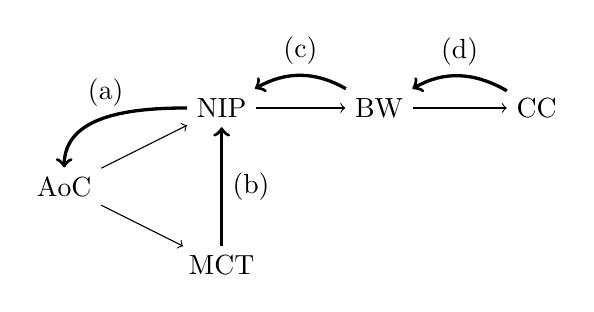
\begin{tikzpicture}
	
	% Draw nodes
	\node (AoC) at (0,0) {AoC};
	\node (MCT) at (2,-1) {MCT};
	\node (NIP) at (2,1) {NIP};
	\node (BW) at (4,1) {BW};
	\node (CC) at (6,1) {CC};
	
	% Draw arcs, what we proved in class
	\draw[->] (AoC) to (MCT);
	\draw[->] (AoC) to (NIP);
	\draw[->] (NIP) to (BW);
	\draw[->] (BW) to (CC);
	
	% Draw arcs, what we will prove here
	\draw[->,very thick,out=180,in=90] (NIP) to node[midway,above] {(a)} (AoC);
	\draw[->,very thick] (MCT) to node[midway,right] {(b)} (NIP);
	\draw[->,very thick,out=150,in=30] (BW) to node[midway,above] {(c)} (NIP);
	\draw[->,very thick,out=150,in=30] (CC) to node[midway,above] {(d)} (BW);
	
	\end{tikzpicture}
	\caption{A directed graph showing the logical implications of the various statements.}\label{fig:theorems}
	\end{center}
	\end{figure}
	
	%%%%%%%%%

	\begin{enumerate}
	
	\item  ~[Wright, A.] Assume that the Nested Interval Property is true.  Hint: use a technique similar to what we used in the Bolzano-Weierstrass Theorem to find our convergent subsequence to prove that the Axiom of Completeness is true.  Let $A$ be the set of interest.  Since we know that $A$ is nonempty and bounded above, construct an interval using an element in $A$ and an upper bound of $A$.  Call this $I_1$.  Cut this interval in half and repeat.  
	
	Since there will be arrows going both ways between NIP and AoC, this argues that NIP and AoC are equivalent assumptions.
	
	\item  ~[Delfosse, D.] Assume that the Monotone Convergence Theorem is true.  Use it to prove that the Nested Interval Property is true.  Hint: start with the collection of nested intervals.  Use the endpoints to construct a monotone sequence, and prove that the limit of that sequence is in the intersection of the nested intervals.  To help, I proved the following lemma.  If you use the lemma, you'll need to prove it, as well.  I used contradiction and a cleverly chosen neighborhood of $a$ in my proof of the lemma.  Be careful, though, you will only be able to use the lemma once.  You might be tempted to use it twice, but it won't be applicable.  Instead, use the Order Limit Theorem.
	
		\begin{lemma}
		If $(a_n)$ is an increasing sequence that converges to $a$, then $a_n \leq a$, for all $n \in \mathbb{N}$.  A similar result holds for decreasing sequences.
		\end{lemma}
	
	We now have that AoC, NIP, and MCT are equivalent assumptions.
	
	\item  ~[Delfosse, D.] Assume that the Bolzano-Weierstrass Theorem is true, and use it to prove that the Nested Interval Property is true.  Hint: this proof will look similar to the proof for (b), but it will be a little harder.  Prove (b) before you attempt (c).
	
	We now have that AoC, NIP, MCT, and BW are equivalent assumptions.
	
	\item  ~[Aitchison, A.] Assume that the Cauchy Criterion is true, and use it to prove that the Bolzano-Weierstrass Theorem is true.  Hint: use the same technique we used to prove the Bolzano-Weierstrass Theorem, but use the intervals to build a subsequence.  Show that such a subsequence is a Cauchy sequence.
	
	We now have that AoC, NIP, MCT, BW, and CC are equivalent assumptions.
	
	\end{enumerate}

%%%%%%%%%%%%%

\end{enumerate}

\end{document}
